%----------------------------------------------------------------------------
\chapter{Tervezés	}
%----------------------------------------------------------------------------
Mindenképp egy blokkdiagrammal kell kezdeni, melyen a rendszer architektúráját ábrázoljuk. Az architektúra a rendszer lényeges komponenseit tartalmazza (hardver, szoftver, felhasználó, internet stb). Például lényeges, hogy a rendszerünk egy adatbázishoz kapcsolódik és mobilos interfésszel rendelkezik, nem lényeges vagy kevésbé lényeges, hogy milyen típusú adatbázist használ.

Itt el lehet indulni a \href{https://en.wikipedia.org/wiki/4\%2B1_architectural_view_model}{Krutchen} féle 4+1 architekturális nézetek iránya felé, mely szinten keretet ad a leírásnak. Érdemes a logikai (logical view) és a folyamat nézeteket (process view) leírni.

Szoftverfejlesztés esetében szoftver architektúráról van szó, melyet komponens diagram segítségével lehet a legjobban ábrázolni.  Amennyiben rendszerünk hardvert is tartalmaz ez is meg kell jelenjen az architektúrán.
Minden lényeges komponens szerepét pár mondatban le kell írni, hogy lehessen a rendszerről egy összképet alkotni. Esetenként pszeudokódot is lehet használni. Ebbe a fejezetbe nem kerül konkrét kód/kódrészlet. 

A szoftverrel kapcsolatos tervek után következhetnek (amennyiben van):
\begin{itemize}
\item Adatbázis terv
\item UI terv - pl. wireframe 
\item Extrák
			\begin{itemize}
			\item Verziókövetés pl. Github, egy branch vagy több. 
			\item Project management - pl. Kanban board segítségével követjük a taskokat.
			\item Rizikó elemzés és tesztelési terv.
		\end{itemize}
\end{itemize}
\begin{figure}[!h]
	\centering
	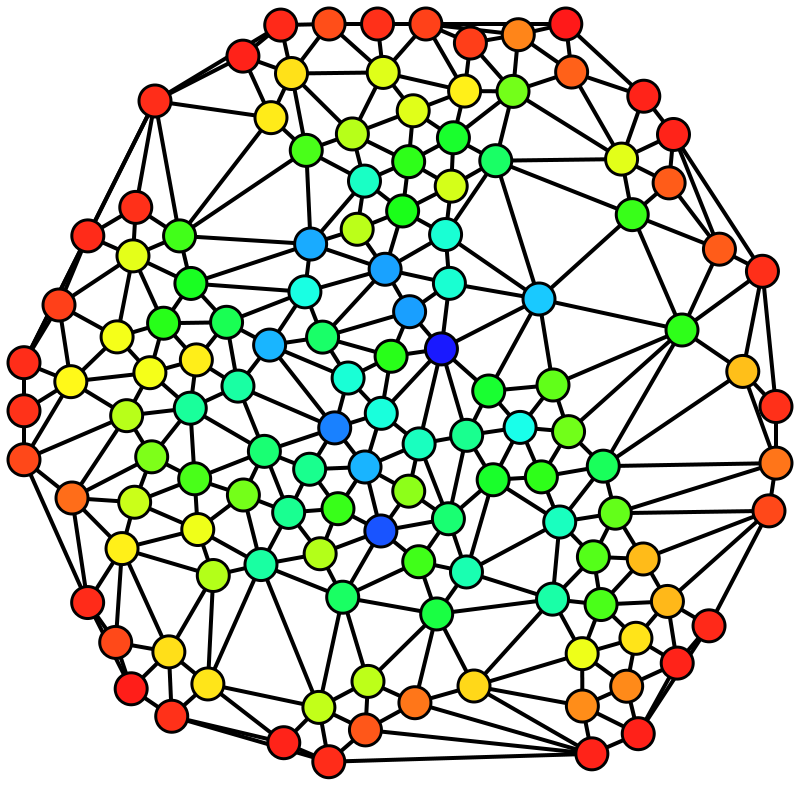
\includegraphics[scale=0.2]{images/graf1}
	\caption{Gr\'af}
\end{figure}


\begin{figure}[!h]
	\centering
	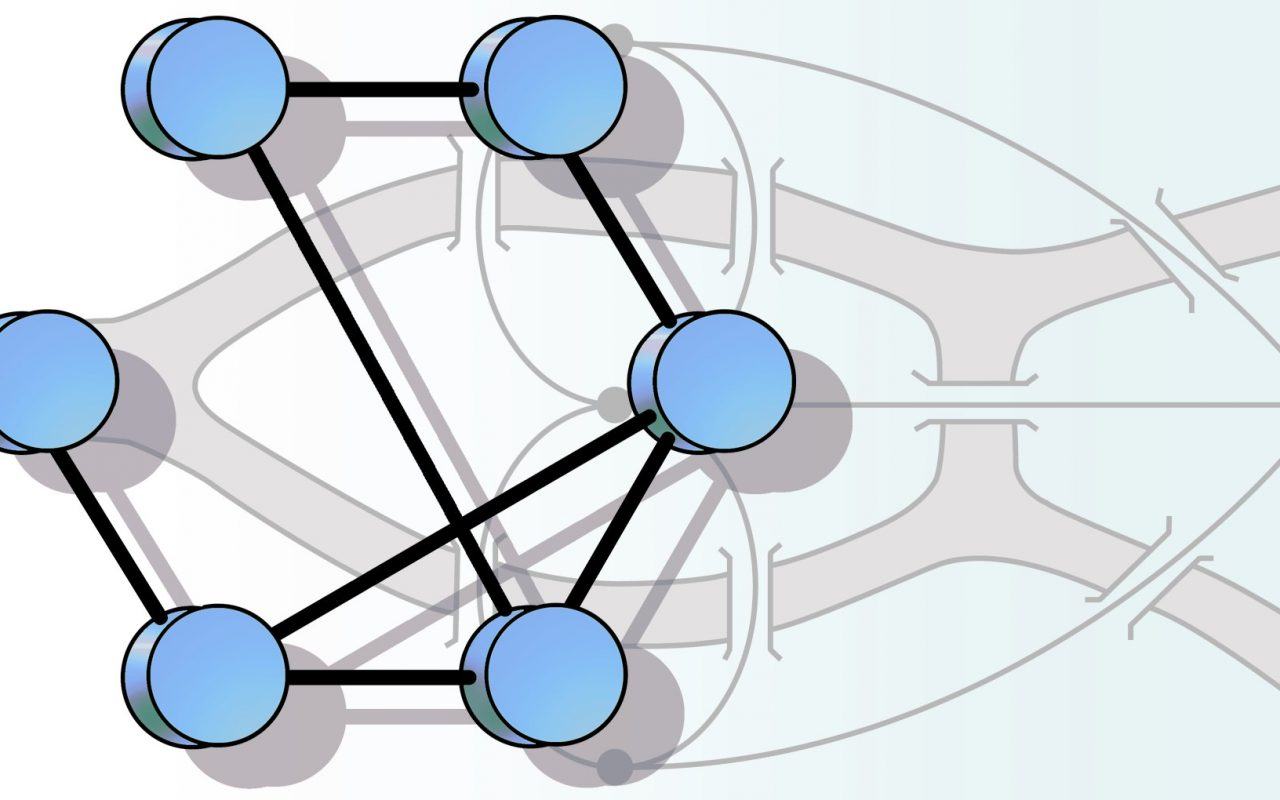
\includegraphics[scale=0.2]{images/graf2}
	\caption{Gr\'af 2}
\end{figure}


\begin{figure}[!h]
	\centering
	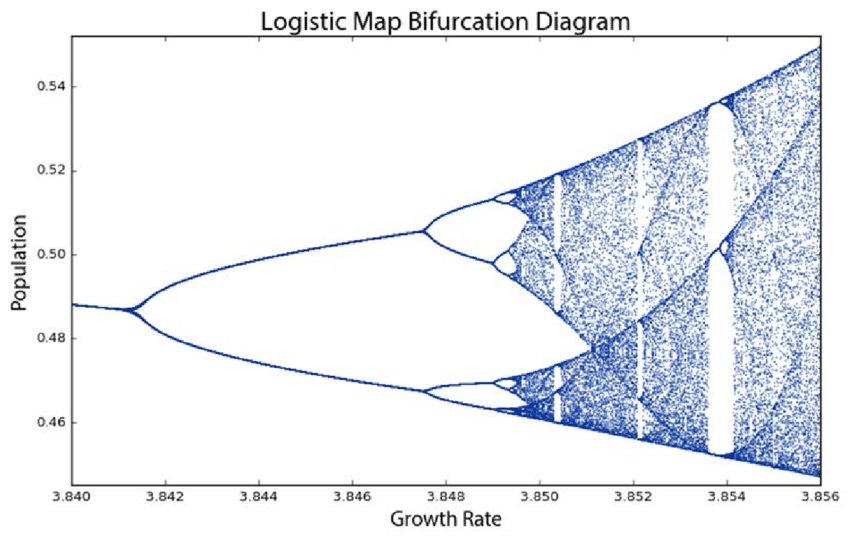
\includegraphics[scale=0.3]{images/kep2}
	\caption{Bifurk\'aci\'os diagram}
\end{figure}



\begin{figure}[!h]
	\centering
	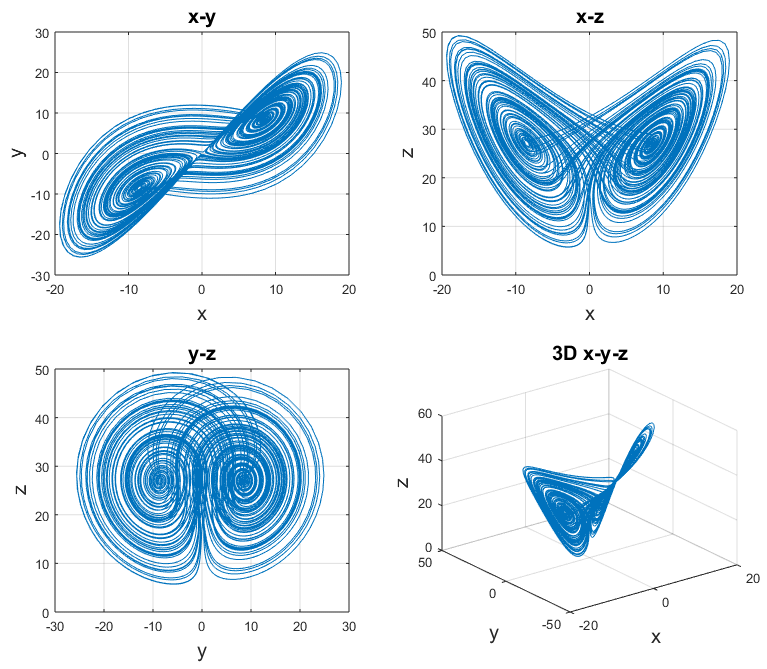
\includegraphics[scale=0.4]{images/kep33}
	\caption{Lorentz attraktor}
\end{figure}